\documentclass[12pt,a4paper]{article}
\usepackage[utf8]{inputenc}
\usepackage{amsmath}
\usepackage{amsfonts}
\usepackage{amssymb}
\usepackage{graphicx}
\graphicspath{ {./img/} }
\usepackage{hyperref}
\usepackage{array}
\usepackage[table]{xcolor}
\usepackage{xcolor,colortbl}
\usepackage{multirow}
\usepackage[a4paper, total={6in, 8in}]{geometry}

\usepackage{titlesec}

\setcounter{secnumdepth}{4}

\titleformat{\paragraph}
{\normalfont\normalsize\bfseries}{\theparagraph}{1em}{}
\titlespacing*{\paragraph}
{0pt}{3.25ex plus 1ex minus .2ex}{1.5ex plus .2ex}

\author{Natale Guadagno, Paolo Patrone}
\title{System Design Document - TecStore}
\renewcommand{\contentsname}{Contenuti}

\usepackage{hyperref}
\hypersetup{
    colorlinks,
        citecolor=blue,
    filecolor=blue,
    linkcolor=blue,
    urlcolor=blue,
    linktocpage
}

\begin{document}

\maketitle
\newpage
\tableofcontents
\newpage
\newgeometry{top=0.5in,bottom=0.5in,right=0.5in,left=0.5in}
\section*{Partecipanti}
\begin{center}
\begin{tabular} {|c|c|}
\hline
\textbf{Nome} & \textbf{Matricola} \\
\hline
Guadagno Natale & 0512106546 \\
Patrone Paolo & 0512106153 \\
\hline
\end{tabular}
\end{center}
\newpage

\section{Introduzione}
\subsection{Scopo del sistema}
Il sistema si propone come interfaccia unificata e semplificata per la gestione di una realtà complessa come un e-commerce.

Le interfacce sono quindi pensate per essere di immediata lettura e accessibili anche per chi ha poca dimestichezza con sistemi informatici.

\subsection{Obiettivi di design}
Per garantire un livello di accessibilità universale sono previsti più test di usabilità per ogni interfaccia, in modo da evidenziare criticità risolvibili. \\
Per facilitare l'utilizzo della piattaforma, ci si è posto anche l'obiettivo di avere un'interfaccia molto reattiva con tempi di risposta molto brevi e molti messaggi di conferma per assicurare gli utenti che le loro operazioni sono state effettuate.

\subsubsection{Criteri prestazionali}
\begin{tabular}{|p{4cm}|p{12cm}|}
\hline
\textbf{Tempi di risposta} & Il sistema si prepone l'obiettivo di essere il più possibile reattivo, ovvero di effettuare la maggioranza delle operazioni semplici come autenticazione, registrazione, risposta ad un ticket in meno di 1s e al più 10s per operazioni più complesse come la ricerca degli articoli. \\
\hline
\textbf{Throughput} & Il sistema si prepone l'obiettivo di gestire anche picchi improvvisi di utenza senza grossi rallentamenti. Sono previsti più webserver con \emph{load balancer} che permettono quindi di gestire molti più utenti. \\
\hline
\textbf{Memorizzazione di dati} & Il sistema utilizzerà un database MySQL per la memorizzazione di dati testuali (informazioni degli utenti, lista degli articoli, ...) e, per evitare di rendere i file del database troppo grandi, i file immagine saranno memorizzati su disco. Tutti questi dati riceveranno dei backup periodici con strategia 3-2-1, ovvero 3 copie dei dati, su 2 dispositivi fisici diversi e almeno 1 copia in un'altra posizione geografica. \\
\hline
\end{tabular}

\subsubsection{Criteri di affidabilità}
\begin{tabular}{|p{4cm}|p{12cm}|}
\hline
\textbf{Robustezza} & L'hardware scelto per il sistema deve essere di livello aziendale e resistente a eventuali problemi hardware come la rottura di un disco fisso, attraverso l'uso di tecnologia RAID, di un alimentatore, con alimentatori ridondanti, alla mancanza di corrente attraverso batterie e sistemi UPS. In nessun caso un singolo crash hardware deve compromettere l'accessibilità al sito.
In più, ci si proteggerà da problematiche software usando versioni del webserver e del sistema operativo testate e senza problemi noti. \\
\hline
\t1extbf{Disponibilità} & Il sistema deve garantire un \emph{uptime} (tempo di attività) di almeno il 99.9\%, ovvero un \textit{downtime} (tempo di inattività) annualizzato di meno di 9 ore. Ciò è cruciale per far sì che l'utenza non venga scoraggiata dall'utilizzo di TecStore come negozio primario, creando perdite potenziali molto alte, soprattutto nei periodi di maggior afflusso di utenza. \\
\hline
\textbf{Tolleranza agli errori} & Il sistema deve garantire l'accessibilità anche in condizioni non ottimali, come il crash di uno dei webserver o un blackout. Ciò è garantito dai componenti ridondanti e dai backup. \\
\hline
\textbf{Sicurezza} & Il sistema deve prevedere tutte le pratiche di sicurezza fondamentali, come l'utilizzo di SSL per la trasmissione dei dati, l'utilizzo di \textit{hashing} e \textit{salt} per le password memorizzate nel database, tutti i dati delle carte di credito e anagrafiche devono essere cifrati prima di essere inseriti nel database utilizzando una cifratura robusta con una chiave che non deve essere esposta pubblicamente per nessun motivo.
In caso di tentativo di accesso a schermate riservate da parte di un utente consumatore o viceversa, ovvero un utente del personale che cerca di accedere al catalogo, deve essere previsto un avviso e un \textit{redirect} ad una pagina correttamente accessibile da quel tipo di utente. \\
\hline
\end{tabular}

\subsubsection{Criteri di manutenzione}
Lo sviluppo del sistema sarà condotto in modo da facilitare l'estensione utilizzando linguaggi e tecnologie standard come HTML5, CSS3, Bootstrap e Java. Il codice deve essere quindi scritto in modo che sia facile intervenire, sia per risolvere eventuali bug, sia per aggiungere nuove funzionalità.

\subsection{Definizioni, acronimi e abbreviazioni}
\begin{itemize}
\item TecStore: nome della piattaforma 
\item Cliente: utente che può acquistare, vendere, richiedere assistenza
\item Centralinista: utente che controlla le vendite e fornisce assistenza ai clienti
\item Magazziniere: utente che controlla la spedizione degli ordini
\item Amministratore catalogo: utente che gestisce le vendite da parte della piattaforma
\item Amministratore personale: utente che gestisce gli account degli altri utenti, fatta eccezione per i clienti
\item DBMS: Database Management System, sistema di gestione di una base di dati
% TODO
\end{itemize}

\subsection{Panoramica}
In questo documento sono descritti in dettaglio:

\begin{itemize}
\item Decomposizione in sottosistemi: in cui viene esposto come il sistema è suddiviso in sottosistemi e come ogni sottosistema interagisce con gli altri.
\item Mapping hardware/software: in cui vengono descritti i requisiti hardware e software su cui il sistema dovrà girare.
\item Gestione dei dati persistenti: in cui viene descritto come i dati verranno memorizzati dal sistema.
\item Controllo degli accessi: in cui vengono descritte le funzionalità messe a disposizione per ogni utente.
\item Condizioni di boundary: in cui verranno descritte le condizioni limite del sistema come avvio, spegnimento, manutenzione e gestione dei fallimenti.
\end{itemize}

\section{Sistema proposto}

\subsection{Panoramica}
L'architettura del sistema è di tipo client/server. Il server resta in attesa di richiesta da parte degli utenti e risponde nel minor tempo possibile.
I motivi per la scelta di un'architettura client/server sono principalmente:
\begin{itemize}
\item Performance: il sistema deve offrire buone prestazioni CPU e ottime prestazioni I/O per garantire una buona reattività.
\item Scalabilità: il sistema è pensato per essere facilmente scalabile orizzontalmente.
\item Affidabilità: il sistema prevede più ridondanze e backup per garantire l'accessibilità da parte degli utenti.
\item Riusabilità: il sistema è facilmente riadattabile ad altre realtà di e-commerce.
\item Tolleranza agli errori: il sistema prevede ridondanze sufficienti per restare operativo anche in caso di criticità di uno o più componenti.
\item Riutilizzo di componenti: il sistema riutilizza più componenti in più punti per semplificare lo sviluppo.
\item Basso costo: il sistema punta a ridurre i costi di sviluppo, manutenzione e gestione utilizzando metodologie di sviluppo e hardware minimale, pur rispettando i requisiti di tolleranza agli errori e affidabilità. 
\end{itemize}

\newpage

\subsection{Controllo degli accessi}

\begin{tabular}{|l|l|l|l|l|l|l|}
\hline
\textbf{} &
  \textbf{Account} &
  \textbf{Assistenza} &
  \textbf{Carrello} &
  \textbf{Ordine} &
  \textbf{Vendita} \\ \hline
\cellcolor[HTML]{C0C0C0}\textbf{\begin{tabular}[c]{@{}l@{}}Utente \\ non autenticato\end{tabular}} &
  {\color[HTML]{34FF34} \begin{tabular}[c]{@{}l@{}}$\checkmark$\\ Solo per\\ registrazione, \\ autenticazione \\ e recupero \\ password \end{tabular}} &
  {\color[HTML]{FE0000} $\times$} &
  {\color[HTML]{FE0000} $\times$} &
  {\color[HTML]{FE0000} $\times$} &
  {\color[HTML]{34FF34} \begin{tabular}[c]{@{}l@{}}$\checkmark$\\ Solo per \\ ricerca e \\ visualizzazione \\ dettagli\end{tabular}} \\ \hline
\cellcolor[HTML]{C0C0C0}\textbf{Cliente} &
  {\color[HTML]{34FF34} \begin{tabular}[c]{@{}l@{}}$\checkmark$\\ Solo per\\ modifica\end{tabular}} &
  {\color[HTML]{34FF34} $\checkmark$} &
  {\color[HTML]{34FF34} $\checkmark$} &
  {\color[HTML]{34FF34} $\checkmark$} &
  {\color[HTML]{34FF34} \begin{tabular}[c]{@{}l@{}}$\checkmark$\\ Fatta eccezione per \\ autorizzazione e  \\ rifiuto di una vendita \\\end{tabular}} \\ \hline
\cellcolor[HTML]{C0C0C0}\textbf{Centralinista} &
  {\color[HTML]{FE0000} $\times$} &
  {\color[HTML]{34FF34} \begin{tabular}[c]{@{}l@{}}$\checkmark$\\ Solo per \\ risposta \\ e chiusura \\ di ticket \\ esistenti\end{tabular}} &
  {\color[HTML]{FE0000} $\times$} &
  {\color[HTML]{FE0000} $\times$} &
  {\color[HTML]{34FF34} \begin{tabular}[c]{@{}l@{}}$\checkmark$\\ Solo per\\ cambiamenti\\ di stato per \\ una vendita\\ ``In attesa"\end{tabular}} \\ \hline
\cellcolor[HTML]{C0C0C0}\textbf{Magazziniere} &
  {\color[HTML]{FE0000} $\times$} &
  {\color[HTML]{FE0000} $\times$} &
  {\color[HTML]{FE0000} $\times$} &
  {\color[HTML]{34FF34} \begin{tabular}[c]{@{}l@{}}$\checkmark$\\ Solo per\\ cambiamenti\\ di stato per \\ ordini \\ e rimborsi \\ ``In attesa"\end{tabular}} &
  {\color[HTML]{FE0000} $\times$} \\ \hline
\cellcolor[HTML]{C0C0C0}\textbf{\begin{tabular}[c]{@{}l@{}}Amministratore \\ Catalogo\end{tabular}} &
  {\color[HTML]{FE0000} $\times$} &
  {\color[HTML]{FE0000} $\times$} &
  {\color[HTML]{FE0000} $\times$} &
  {\color[HTML]{FE0000} $\times$} &
  {\color[HTML]{34FF34} \begin{tabular}[c]{@{}l@{}}$\checkmark$\\ Fatta eccezione per \\ autorizzazione e  \\ rifiuto di una vendita \\\end{tabular}} \\ \hline
\cellcolor[HTML]{C0C0C0}\textbf{\begin{tabular}[c]{@{}l@{}}Amministratore \\ Personale\end{tabular}} &
  {\color[HTML]{34FF34} \begin{tabular}[c]{@{}l@{}}$\checkmark$\\ Solo per \\ creazione \\ e modifica \\ di account \\ di dipendenti \end{tabular}} &
  {\color[HTML]{FE0000} $\times$} &
  {\color[HTML]{FE0000} $\times$} &
  {\color[HTML]{FE0000} $\times$} &
  {\color[HTML]{FE0000} $\times$} \\ \hline
\end{tabular}

\newgeometry{top=0.5in,bottom=0.5in,right=0.5in,left=0.5in}

\section{Decomposizione in sottosistemi}
Per realizzare il sistema è prevista un'architettura Three-Tier, con divisione in tre sottosistemi principali:
\begin{itemize}
\item Presentation Layer, composto da tutte le interfacce riservate agli utenti finali.
\item Application Layer, composto da tutti gli oggetti che si occupano di gestire e manipolare le operazioni e i dati che provengono dal Presentation Layer.
\item Storage Layer, composto dai sistemi di memorizzazione dei dati persistenti e dalle procedure di memorizzazione e recupero di dati. 
\end{itemize}

\subsection{Presentation Layer}
Il Presentation Layer si suddivide a sua volta in:

\begin{itemize}
\item Sottosistema cliente, che include quasi tutte le funzionalità del sito, come registrazione, autenticazione, ricerca, aggiunta al carrello, acquisto, creazione e risposta a \emph{ticket}, vendita di articoli.
\item Sottosistema centralinista, che si occupa dei \emph{ticket} e di autorizzare le vendite dei clienti.
\item Sottosistema magazziniere, che si occupa di confermare la spedizione degli ordini e confermare la ricezione degli articoli per i quali i clienti richiedono un rimborso.
\item Sottosistema amministratore personale, che si occupa di gestire l'inserimento e la modifica degli account riservati ai dipendenti della piattaforma.
\item Sottosistema amministratore catalogo, che si occupa di gestire l'inserimento e la modifica degli articoli venduti dalla piattaforma.
\end{itemize}

\subsection{Application Layer}
L'Application Layer si suddivide a sua volta in:

\begin{itemize}
\item GestioneAccount, che contiene tutte le operazioni riguardanti gli account degli utenti come registrazione, modifica e autenticazione.
\item GestioneAssistenza, che contiene tutte le operazioni riguardanti i \emph{ticket} come creazione, risposta e chiusura.
\item GestioneCarrello, che contiene tutte le operazioni riguardanti il carrello come aggiunta e rimozione.
\item GestioneOrdine, che contiene tutte le operazioni riguardanti gli ordini come creazione, annullamento, rimborso.
\item GestioneVendita, che contiene tutte le operazioni riguardanti le vendite, sia dei clienti che della piattaforma, come creazione, rimozione, visualizzazione e modifica.
\end{itemize}

\subsubsection{Utente non autenticato}

\begin{center}
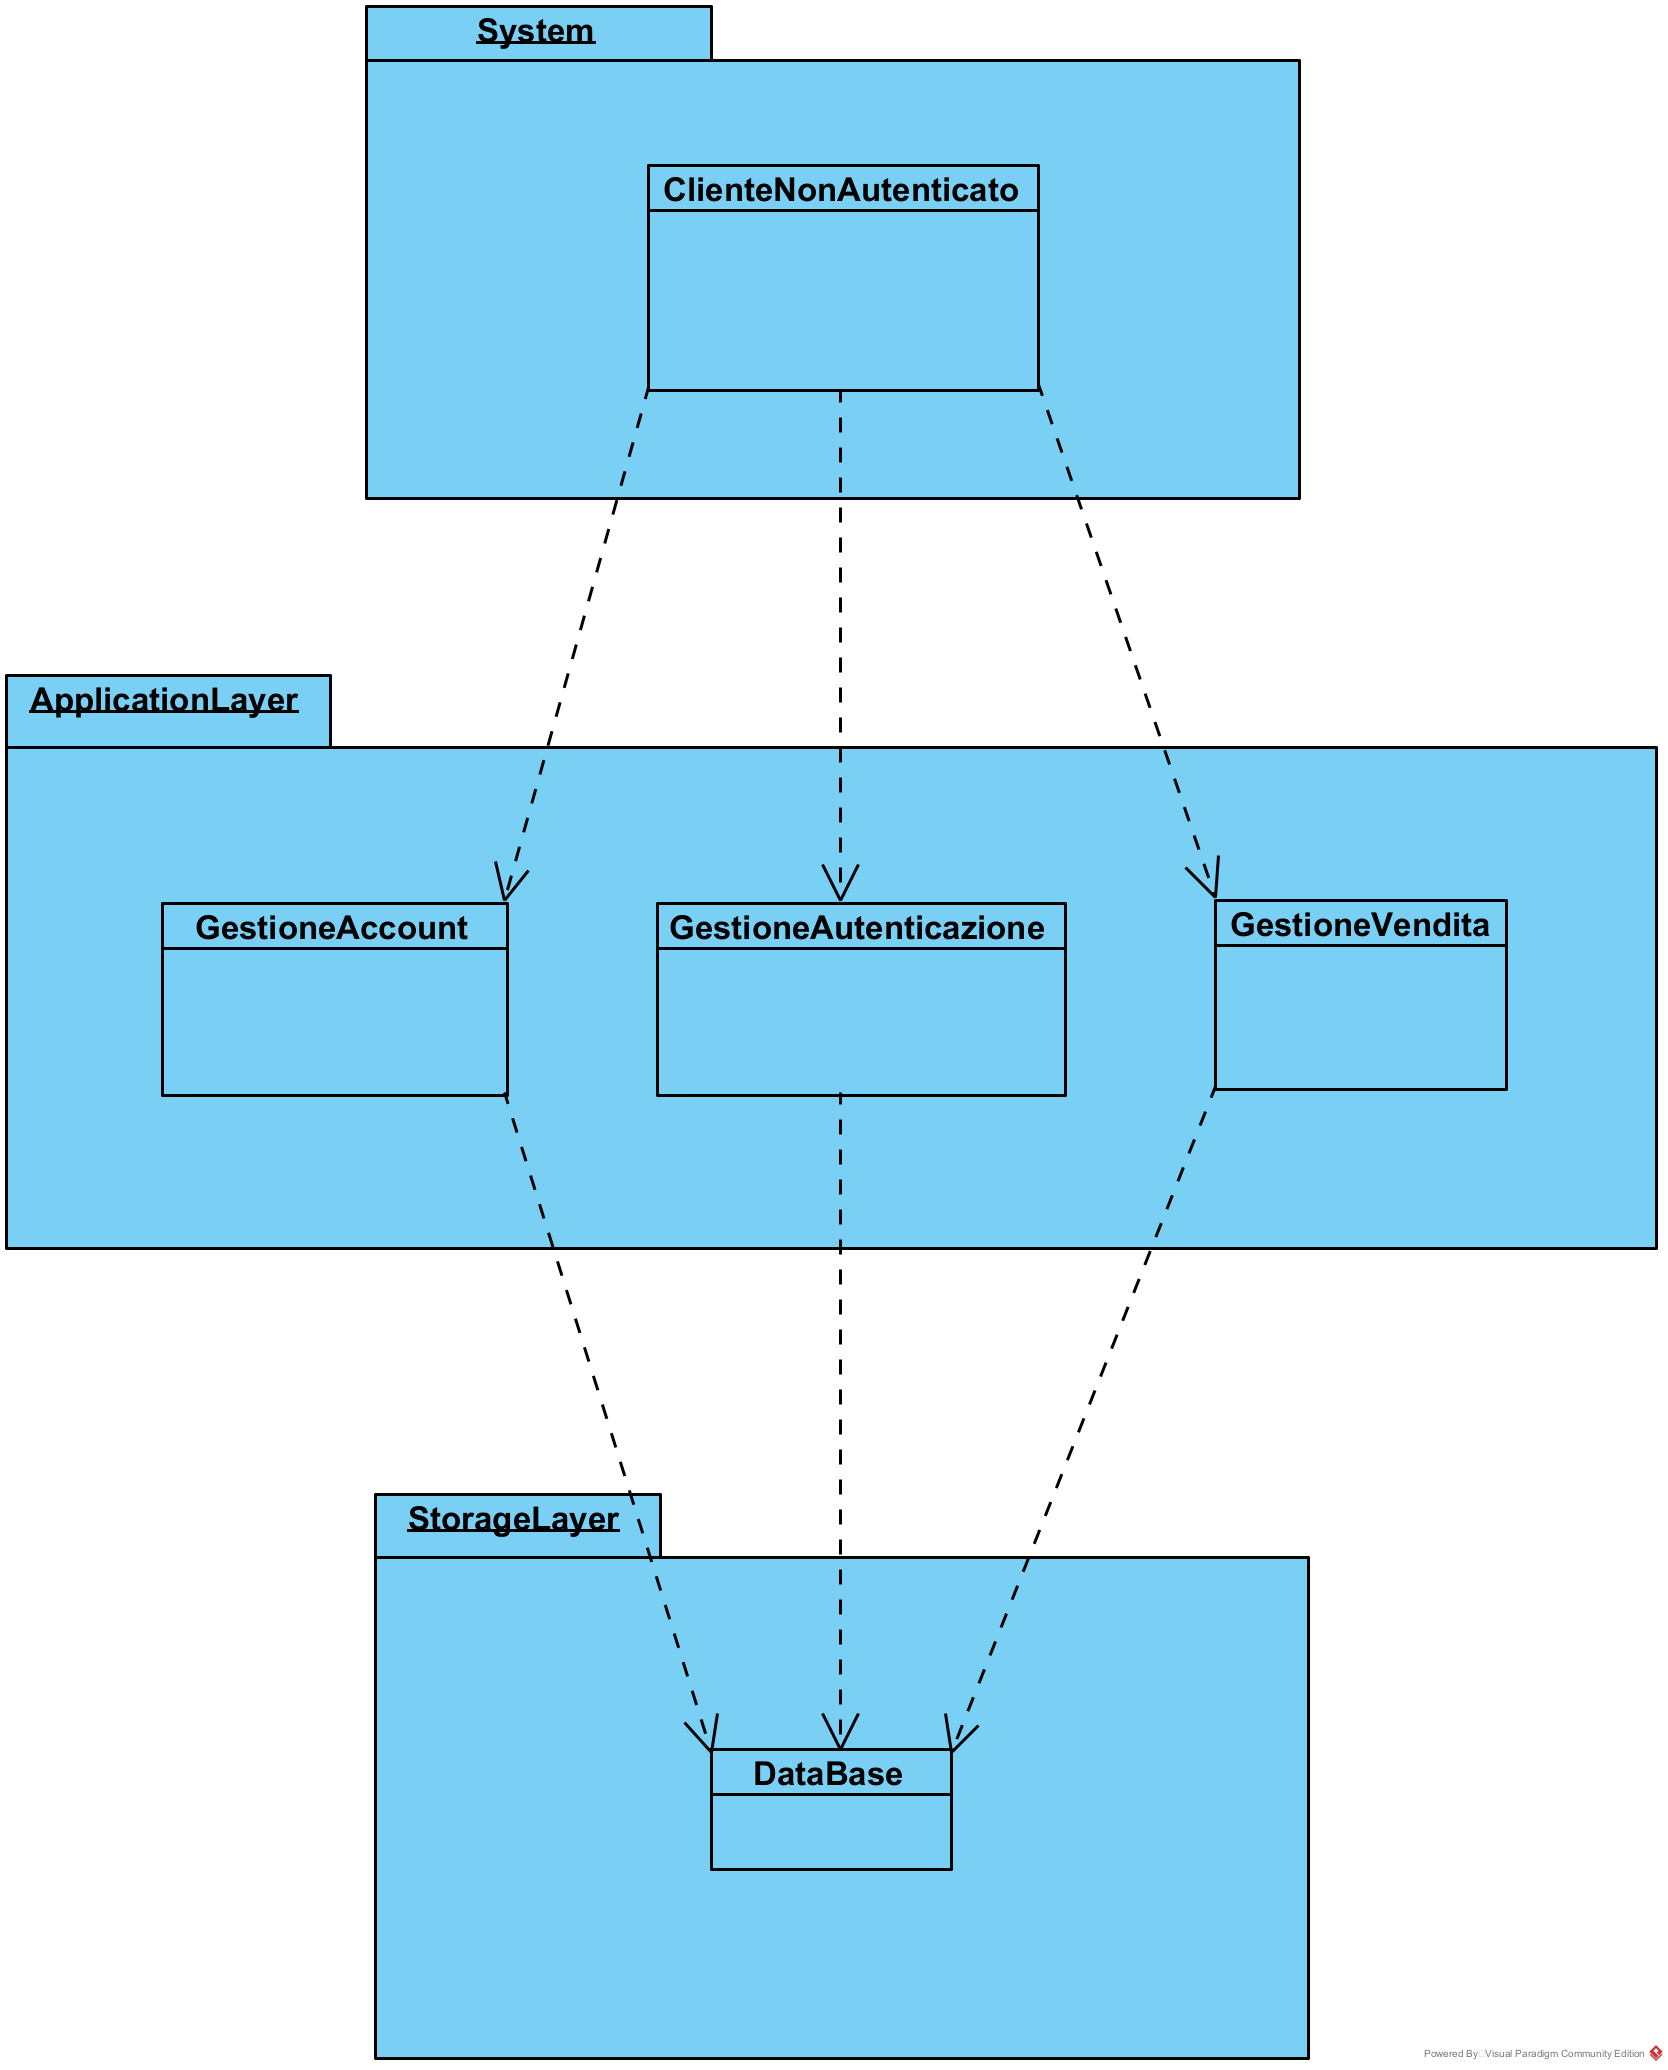
\includegraphics[height=0.34\textheight]{UtenteNonAutenticato}
\end{center}

\begin{itemize}
\item un utente non autenticato può accedere al sottosistema Account soltanto per autenticarsi, recuperare la password e per registrarsi.
\item un utente non autenticato può accedere al sottosistema Vendita soltanto per ricercare un articolo e per visualizzare i dettagli di un articolo.
\end{itemize}

\newpage

\subsubsection{Cliente}
\begin{center}
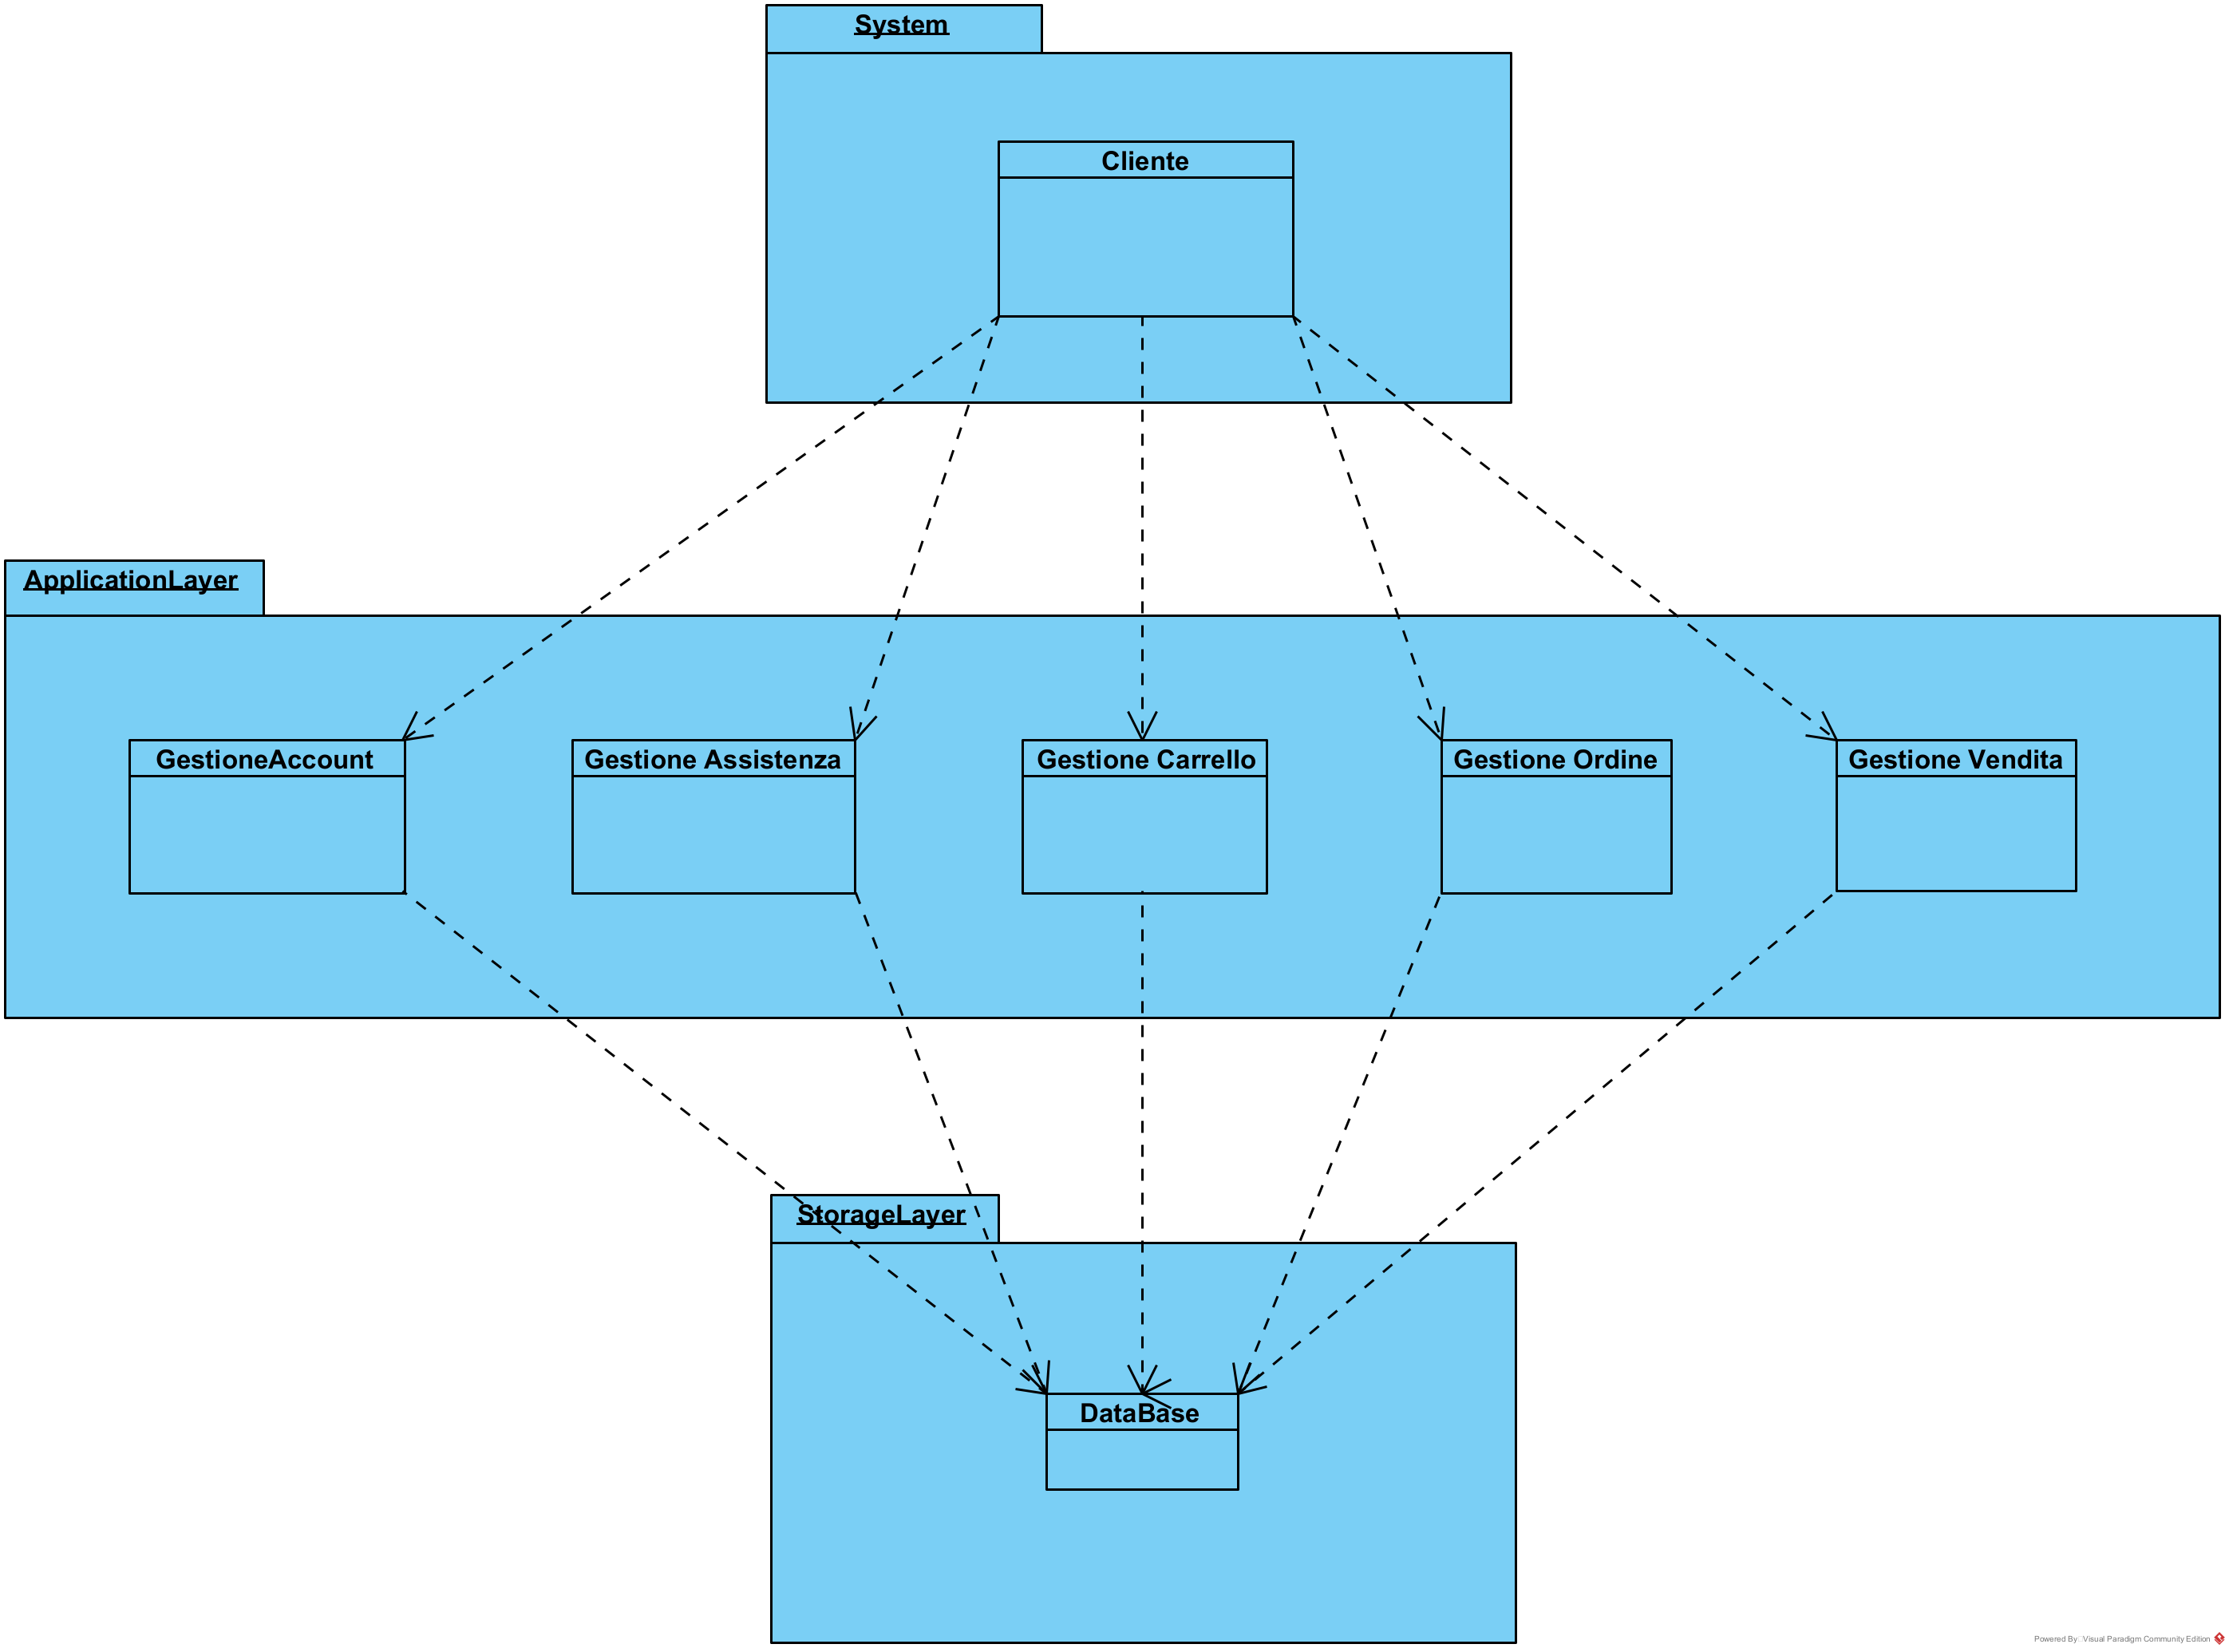
\includegraphics[height=0.34\textheight]{Cliente}
\end{center}
\begin{itemize}
\item un cliente autenticato può accedere al sottosistema Account soltanto per la modifica delle proprie informazioni come indirizzo, dati della carta di credito o password.
\item un cliente autenticato può accedere al sistema assistenza per effettuare tutte le operazioni previste per il sottosistema Assistenza, quindi creazione, risposta e chiusura di un ticket.
\item un cliente autenticato può accedere al sistema assistenza per effettuare tutte le operazioni previste per il sottosistema Carrello, quindi inserimento e rimozione di articoli.
\item un cliente autenticato può accedere al sistema assistenza per effettuare tutte le operazioni previste per il sottosistema Ordine, quindi creazione, annullamento e rimborso.
\item un cliente autenticato può accedere al sistema assistenza per effettuare tutte le operazioni previste per il sottosistema Vendita, quindi creazione, modifica e annullamento, fatta eccezione per le operazioni riservate come autorizzazione e rifiuto vendita, che sono di competenza dei centralinisti. 
\end{itemize}

\subsubsection{Centralinista}
\begin{center}
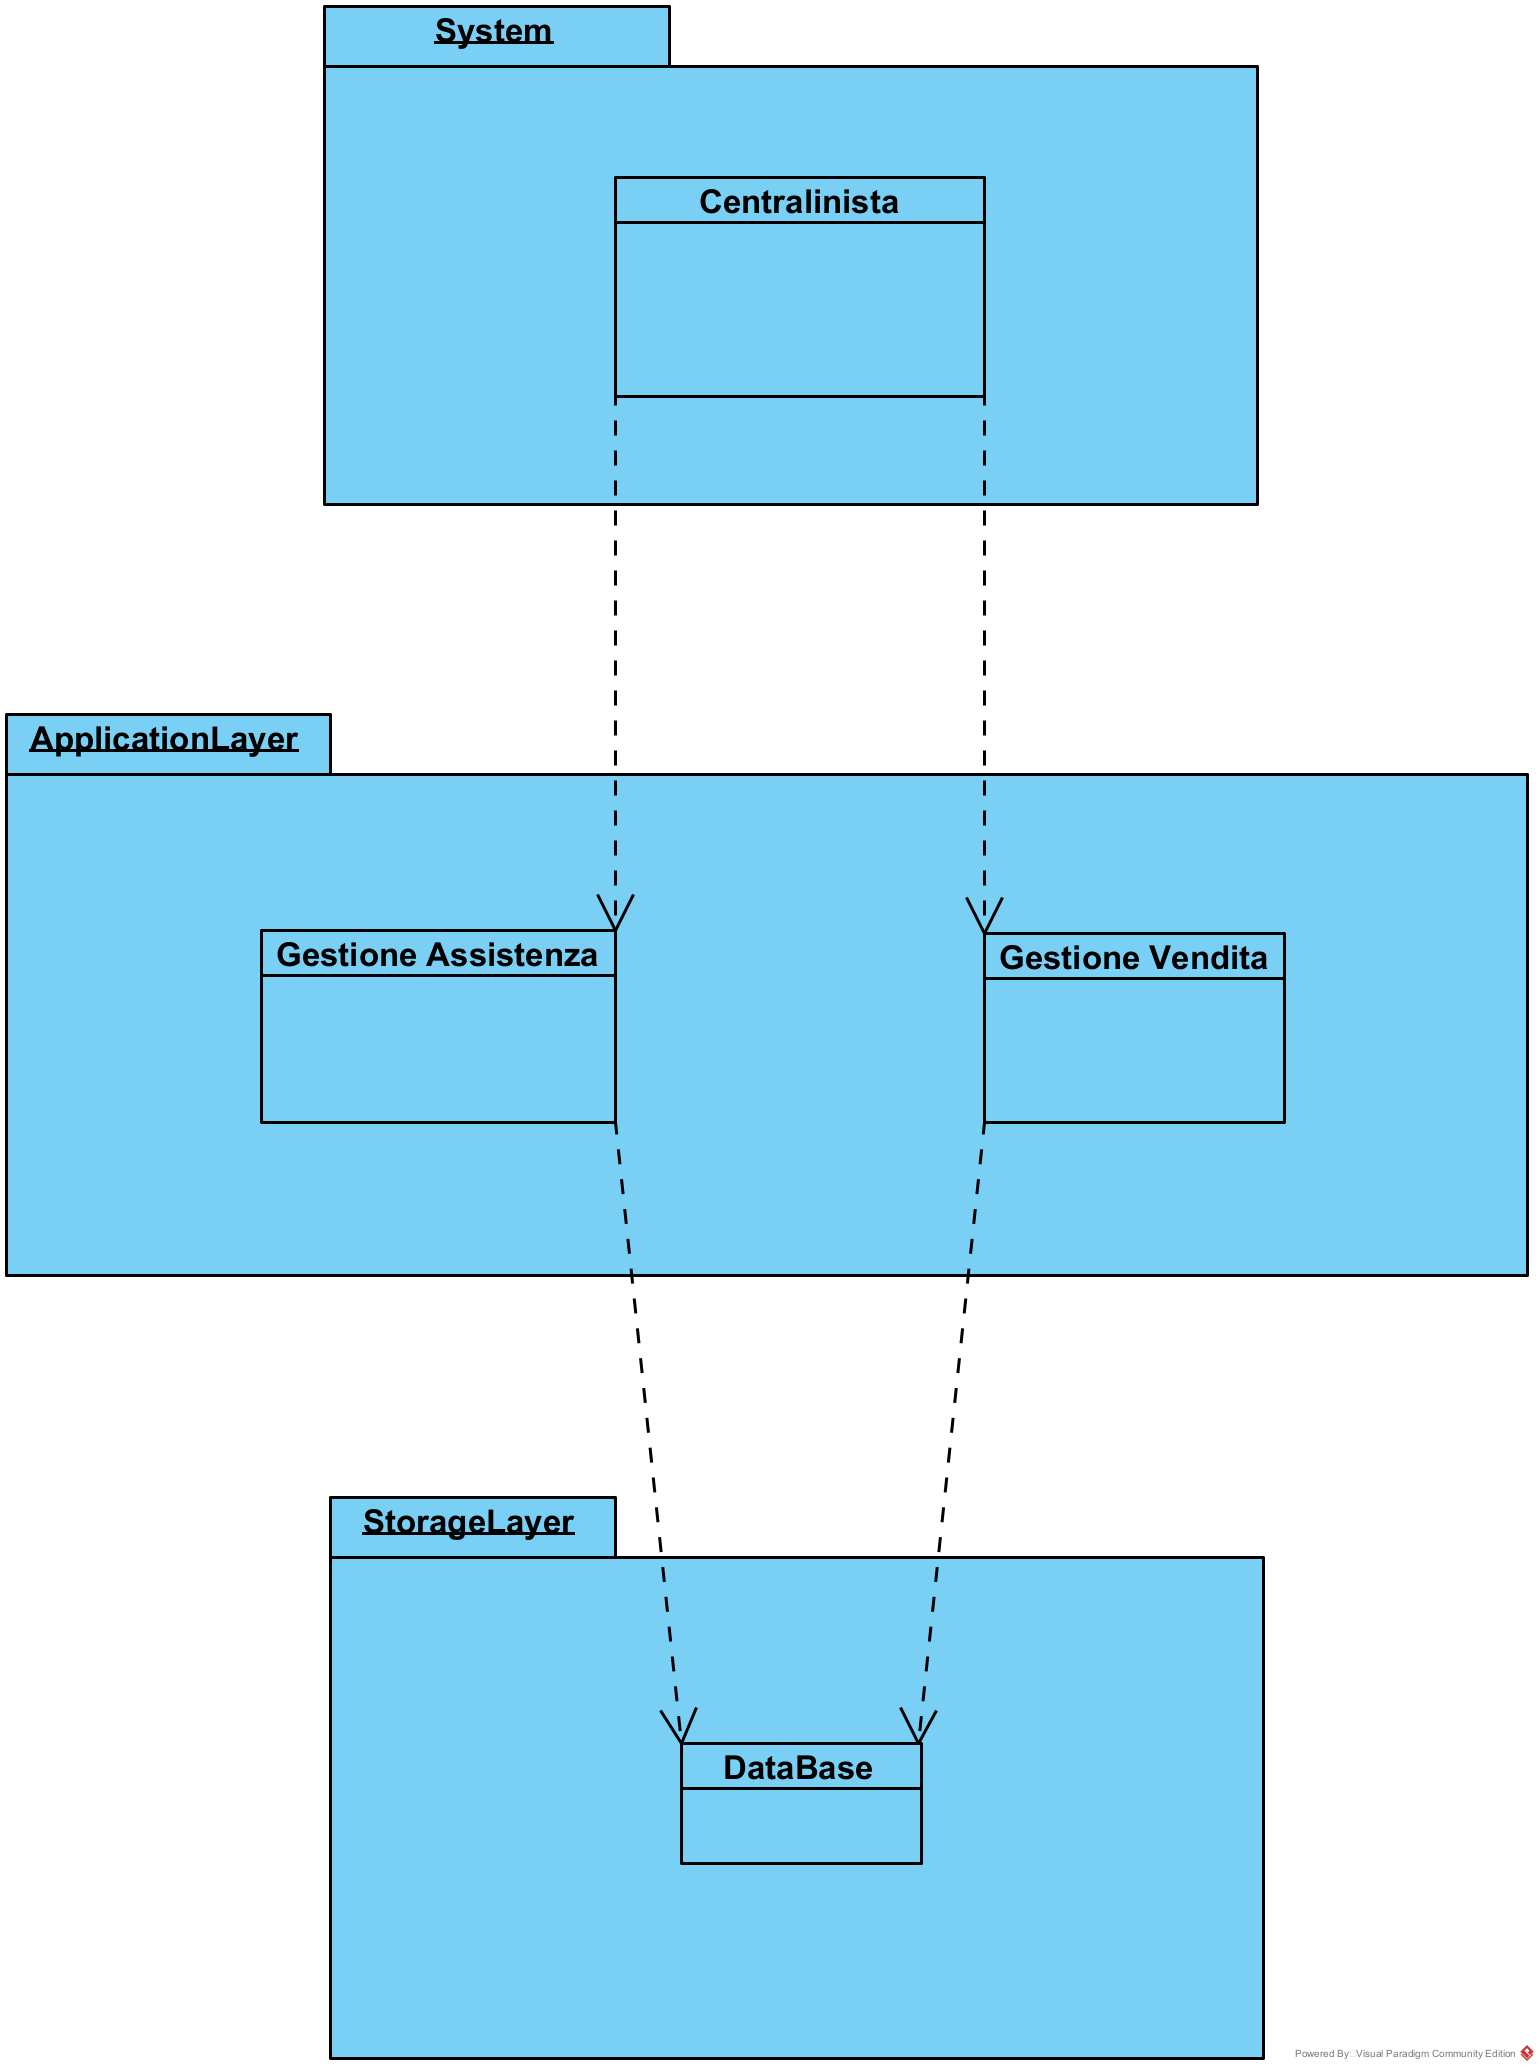
\includegraphics[height=0.34\textheight]{Centralinista}
\end{center}

\begin{itemize}
\item Un centralinista ha accesso al sottosistema Assistenza per le operazioni di risposta e chiusura di un ticket, ma non può crearne uno nuovo.
\item un centralinista ha accesso al sottosistema Vendita solo per l'autorizzazione o il rifiuto di una vendita immessa da un cliente.
\end{itemize}

\subsubsection{Magazziniere}
\begin{center}
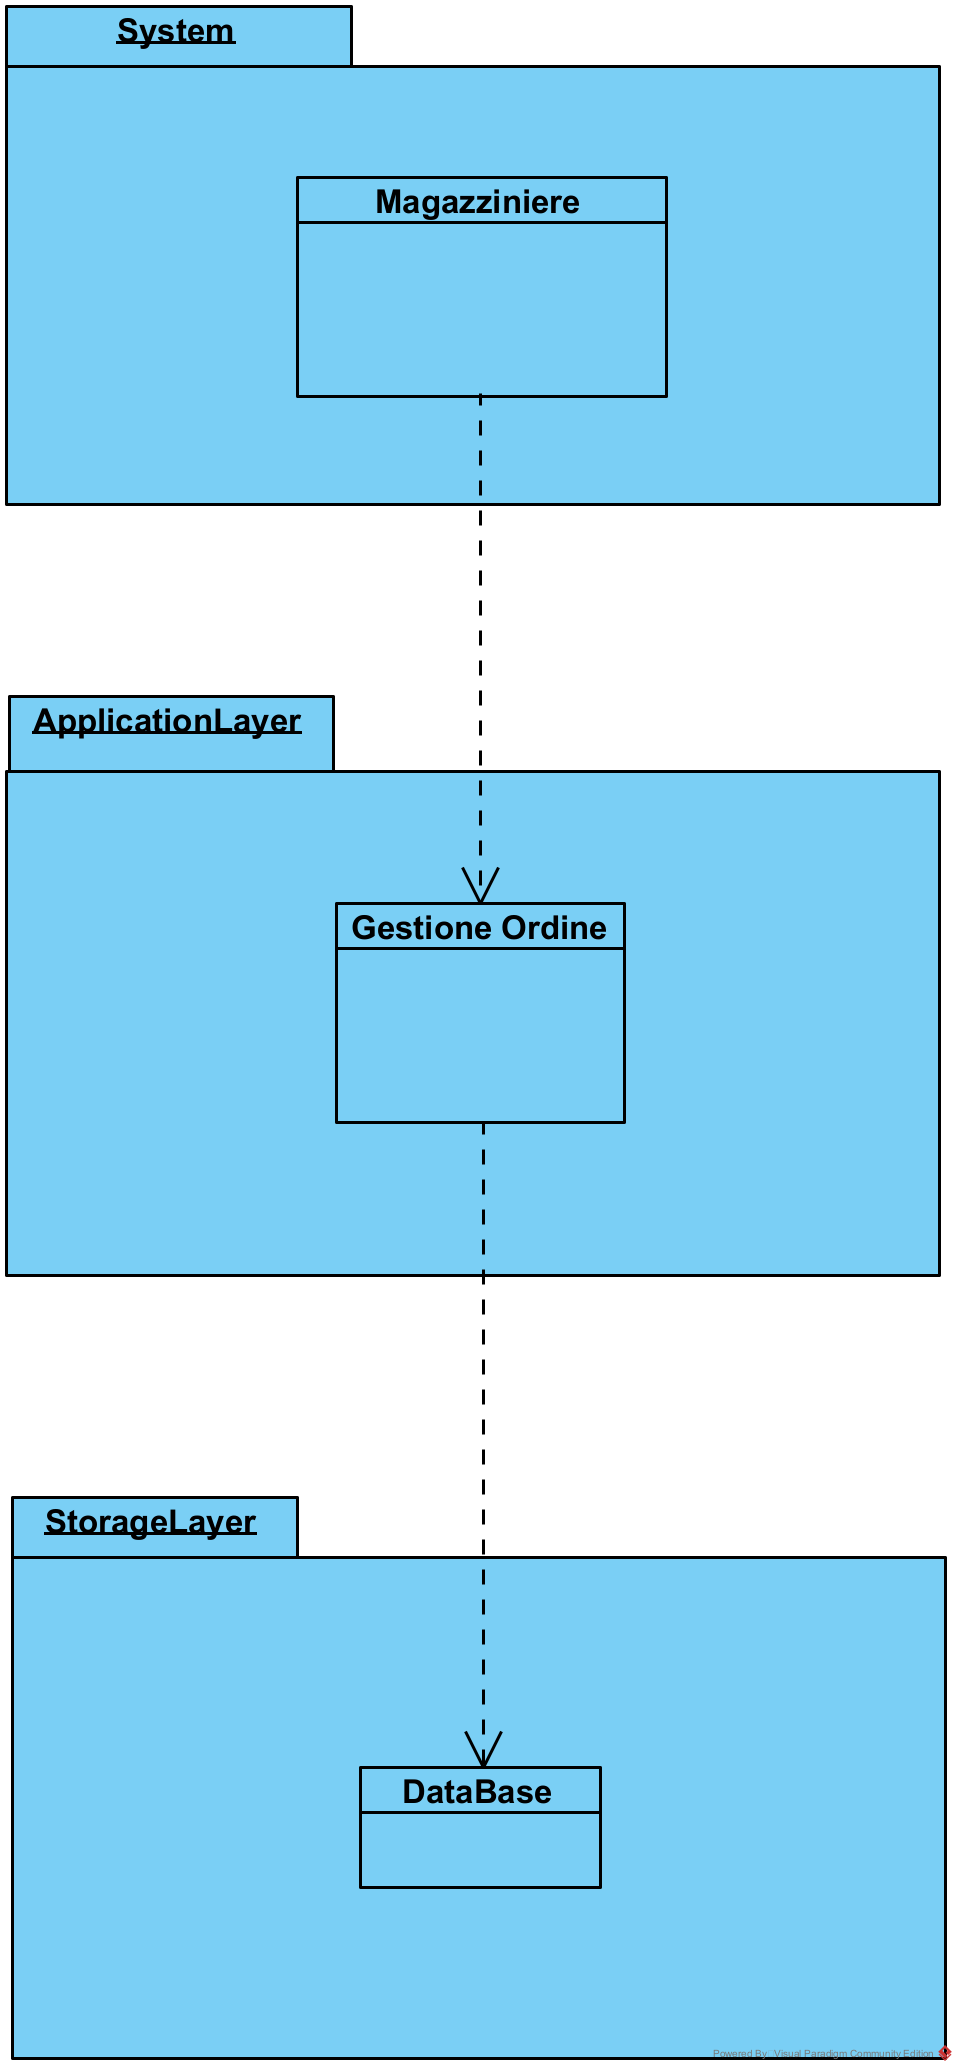
\includegraphics[height=0.34\textheight]{Magazziniere}
\end{center}

\begin{itemize}
\item Un magazziniere ha accesso al sottosistema Ordine solo per il cambio di stato di un ordine in seguito ad una spedizione o al cambio di stato di un rimborso in seguito al ricevimento dell'articolo.
\end{itemize}

\subsubsection{Amministratore Personale}
\begin{center}
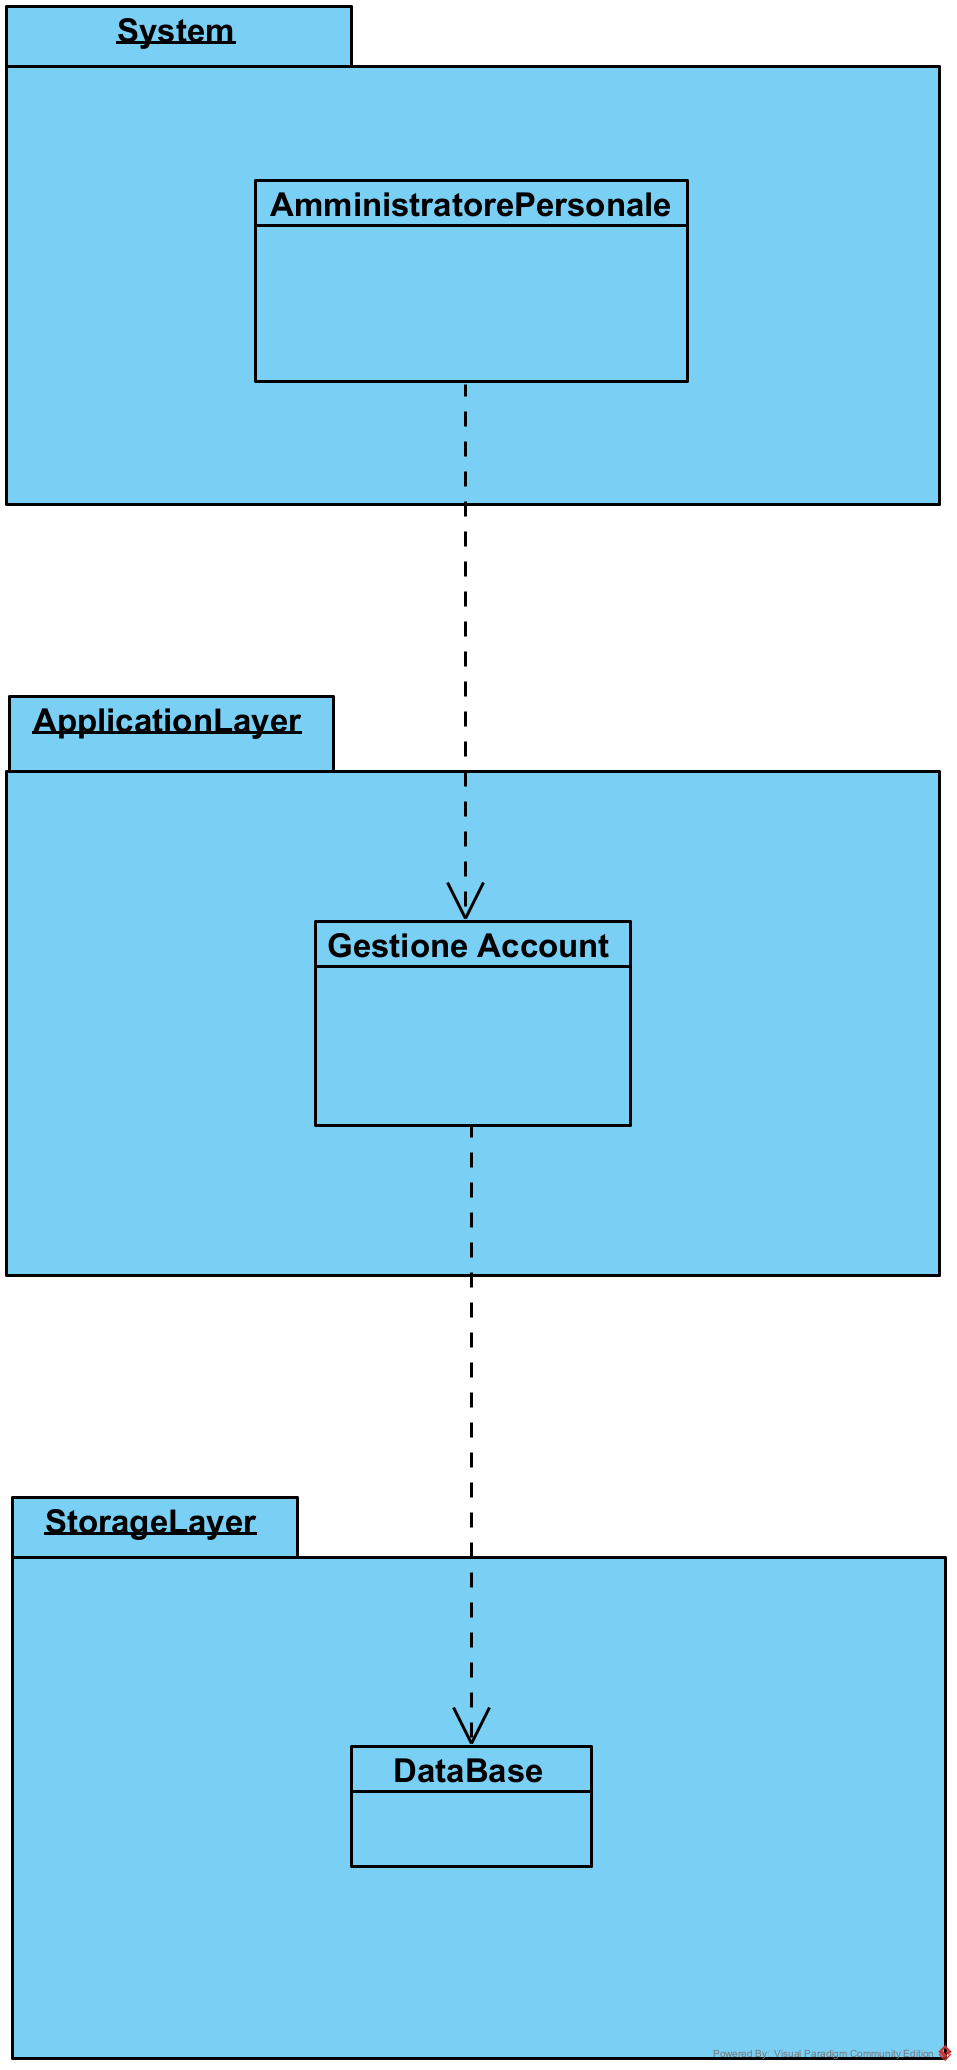
\includegraphics[height=0.34\textheight]{AmministratorePersonale}
\end{center}

\begin{itemize}
\item Un amministratore del personale ha accesso al sottosistema Account solo per l'inserimento e la modifica degli account dei dipendenti.
\end{itemize}

\subsubsection{Amministratore Catalogo}
\begin{center}
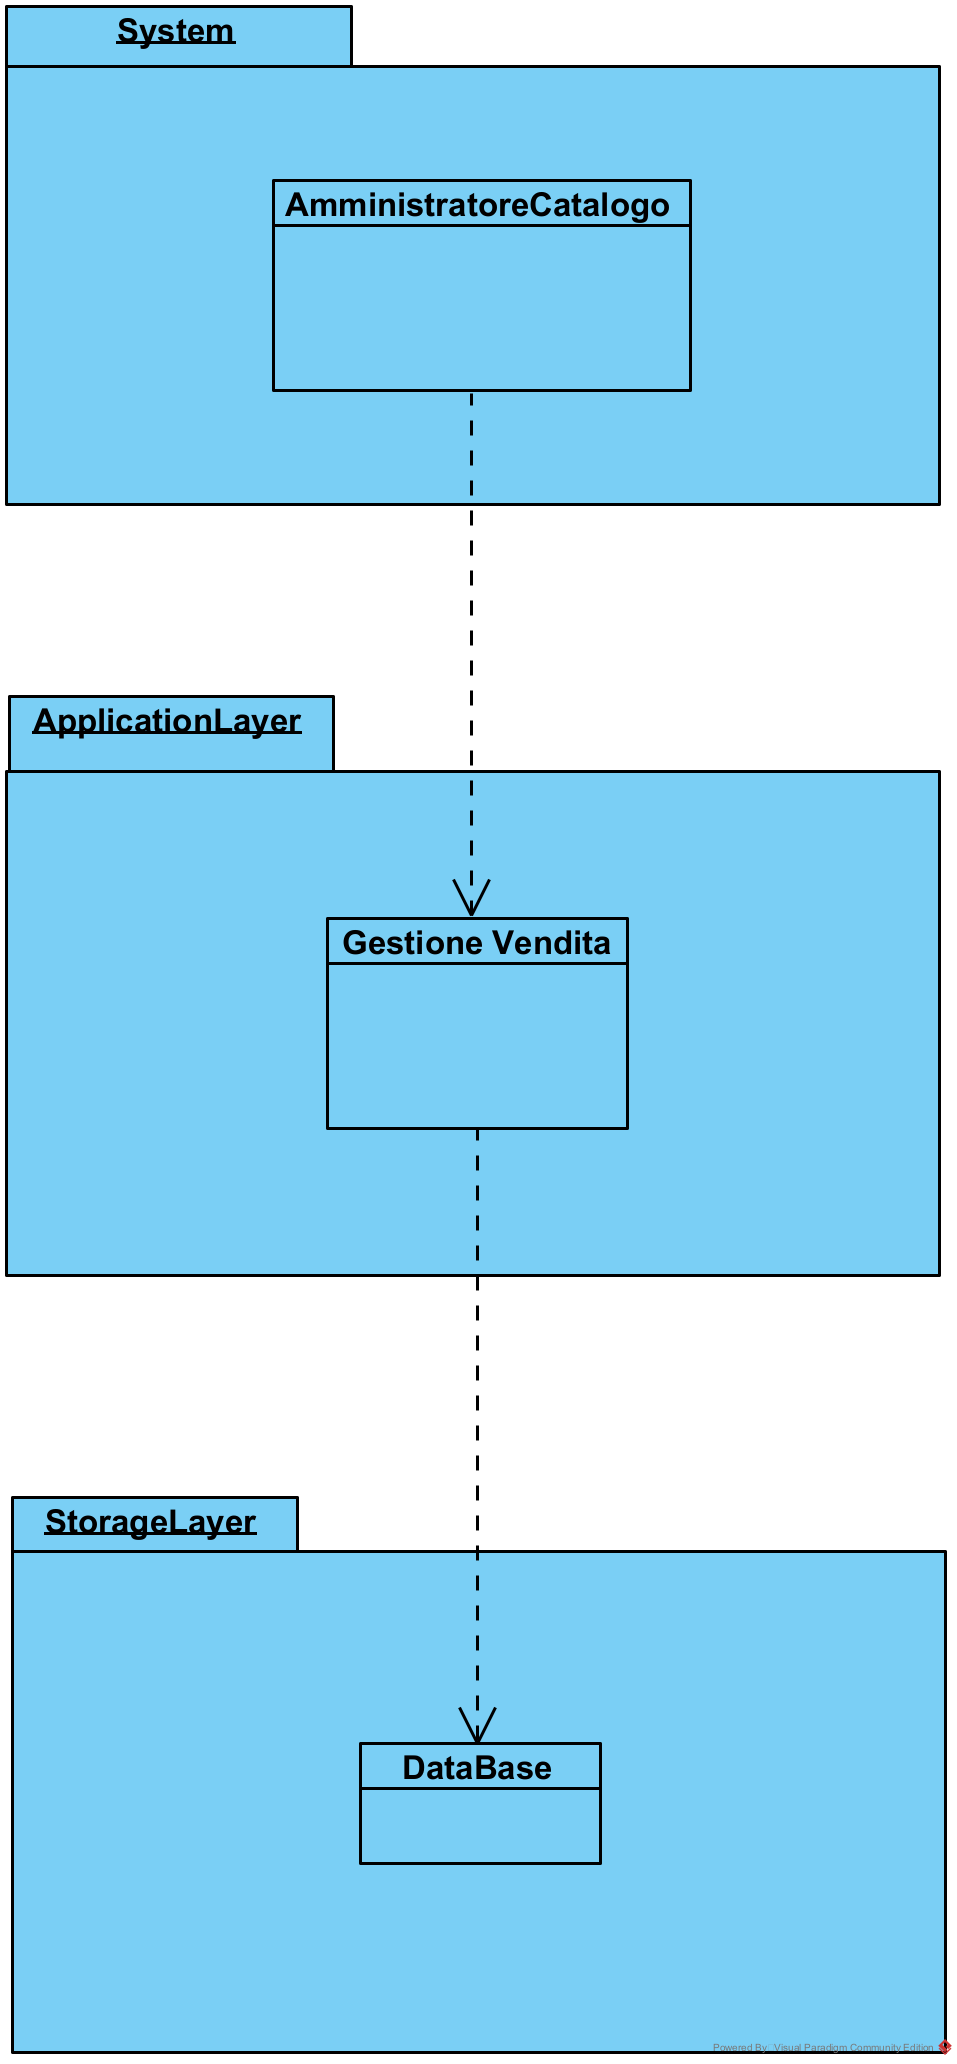
\includegraphics[height=0.34\textheight]{AmministratoreCatalogo}
\end{center}

\begin{itemize}
\item Un amministratore del catalogo ha accesso al sottosistema Vendita solo per l'inserimento e la modifica di articoli.
\end{itemize}

\subsection{Mapping Hardware/Software}
\begin{center}
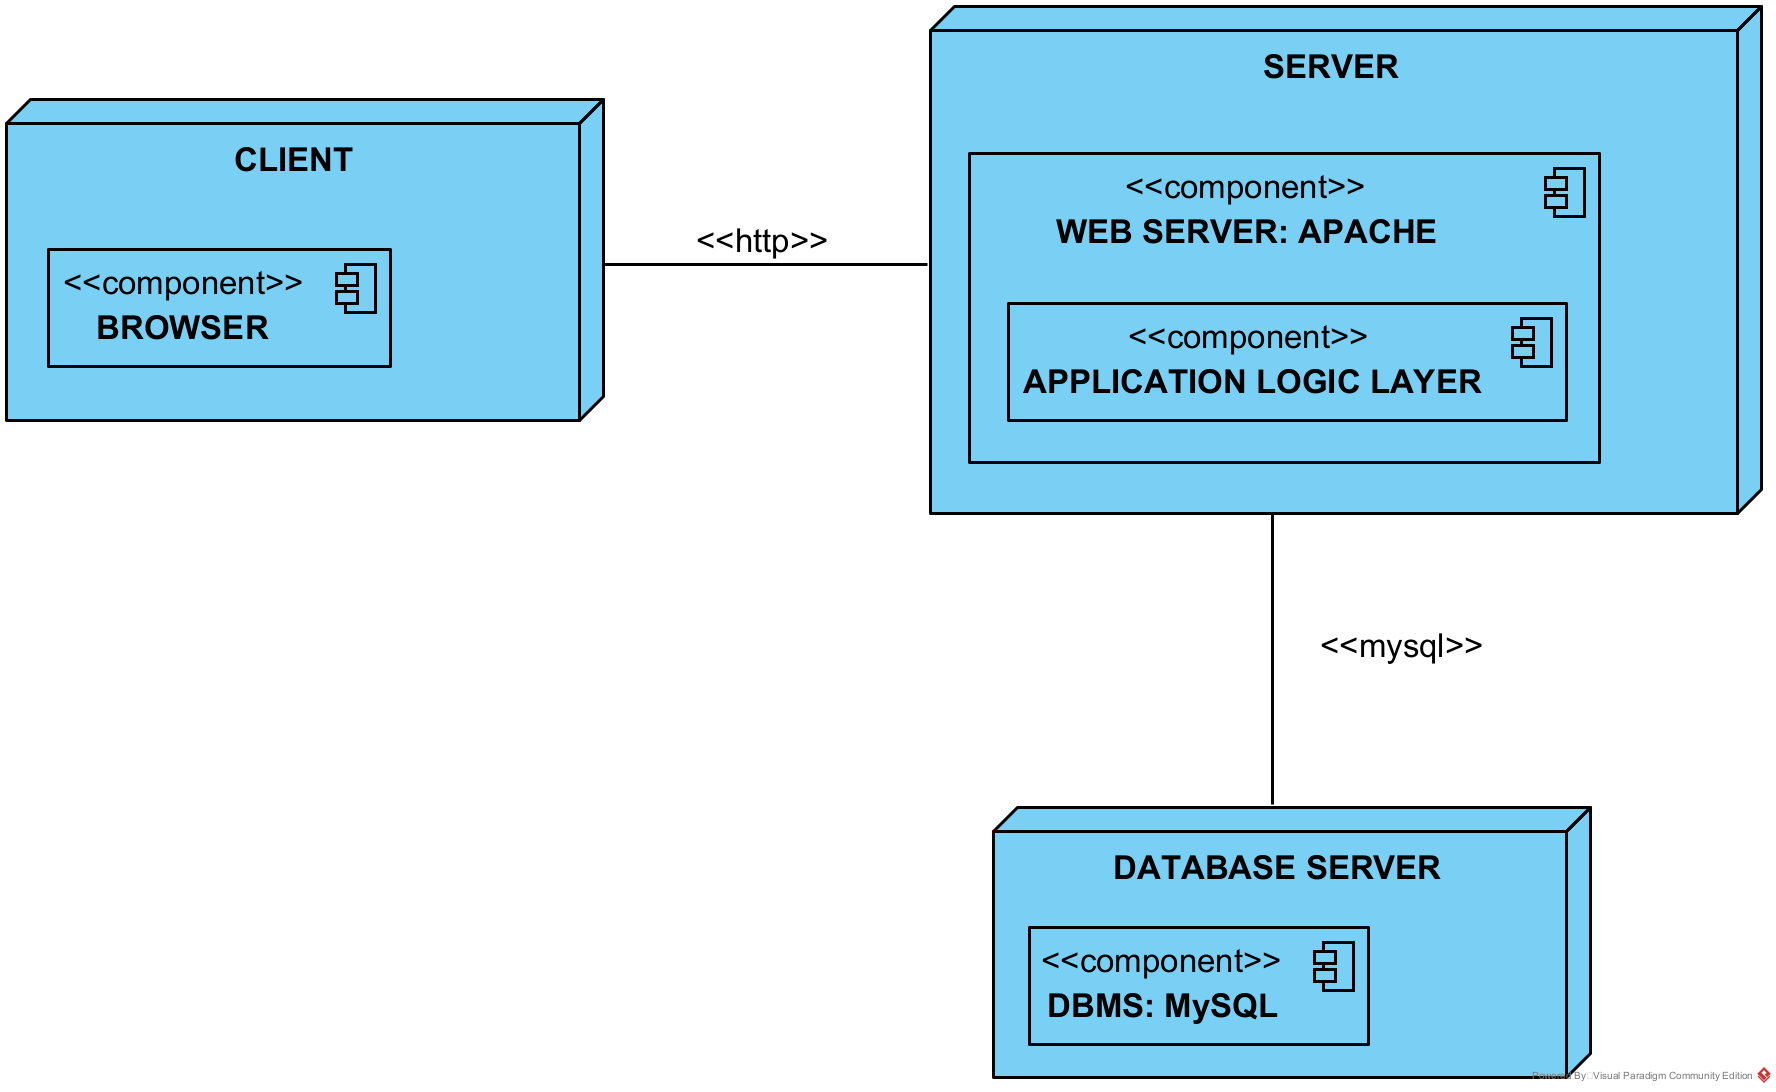
\includegraphics[height=0.34\textheight]{MappingHardWare_Software}
\end{center}

\begin{itemize}
\item \textbf{Webserver}: Il webserver utilizzato è Apache Tomcat % TODO versione
\item \textbf{Interface Layer}: Gli utenti si interfacciano con il sistema mediante un comune browser HTTP.
\item \textbf{Application Layer}: Tutte le funzionalità del sistema sono implementate in linguaggio Java utilizzando il componente Java Servlet.
\item \textbf{Storage Layer}: Il sistema utilizza il DMBS MariaDB per la memorizzazione dei dati testuali (informazioni degli account, storico ordini, lista vendite, ...) e il filesystem ext4 per memorizzare le foto degli articoli.
\end{itemize}

\newpage

\subsubsection{Class Diagram}
\begin{center}
\includegraphics[width=\textwidth]{../../RAD/img/diagrammadiclasse}
\end{center}

% tabelle SQL?

\newpage

\section{Boundary Condition}
\subsection{Avvio del sistema}
Per l'avvio del sistema è necessario che almeno un'istanza del webserver e del database siano attive.
All'avvio del sistema operativo i due servizi devono essere quindi avviati automaticamente senza intervento manuale.

\subsection{Spegnimento del sistema}
Nell'eventualità in cui sia richiesto che uno dei server vada offline per qualsiasi motivo, deve essere previsto che almeno un'altra istanza del DBMS e del webserver siano attive. Se non lo sono, l'intero sistema può andare offline per un tempo indefinito.

\subsection{Fallimenti del sistema}
Ci sono più scenari in cui il sistema può subire un fallimento. Partendo da quelli non critici:
\begin{enumerate}
\item Fallimento o spegnimento di uno dei server, che può essere causato dalla perdita di connessione ad internet, blackout o un guasto hardware. Se le ridondanze sono attive, riduce le prestazioni del sistema se ci sono più utenti, ma non è un errore critico.
\item Fallimento, spegnimento o perdita di connessione ad internet del dispositivo client, che deve essere correttamente gestito, quindi evitando, ad esempio, ordini duplicati. Il sistema deve mantenere le informazioni informazioni inserite dall'utente fino a quel momento.
\end{enumerate}

Tra i fallimenti critici ci sono:

\begin{enumerate}
\item Fallimento di uno o più server, sia per motivi hardware che software, che può essere fatale nel caso non ci siano più ridondanze sufficienti a gestire tutta l'utenza, peggiorando le prestazioni del sito al punto in cui può fallire del tutto. È necessario un intervento manuale per ripristinare almeno un'istanza del webserver e del DBMS per ripristinare la funzionalità del sistema.
\item Fallimento dei backup, che può succedere in caso di spazio insufficiente per memorizzare i dati e che può rendere il sito inoperabile in seguito a un fallimento totale. È un errore che nella migliore delle ipotesi fa perdere qualche giorno di informazioni e, in casi catastrofici, può far perdere tutte le informazioni memorizzate nel sistema. L'ultimo caso è irrecuperabile.
\end{enumerate}


\subsection{Casi d'uso}
\subsubsection{Configurazione di un nuovo sistema}
\begin{tabular}{|>{\columncolor[gray]{0.8}}c|p{12cm}|}
\hline
\textbf{ID} & UC1 NuovoServer \\
\hline
\textbf{Descrizione} & Un sysadmin aggiunge un nuovo server.  \\
\hline
\textbf{Partecipanti} & Sysadmin \\
\hline
\textbf{Condizione d'ingresso} & Un sysadmin ha accesso ad un nuovo server. \\
\hline
\textbf{Flusso di eventi} &
\begin{minipage}{12cm}
\begin{tabular}{p{5.5cm} p{5.5cm}}
\textbf{Sysadmin} & \textbf{Sistema} \\
Dà i comandi per installare Java, Tomcat e MariaDB. \\
	& Installa i software richiesti. \\
Utilizza lo script ad-hoc per la configurazione di un nuovo server. \\
	& Scarica e configura i sorgenti nelle cartelle opportune e imposta i servizi per essere avviati automaticamente all'avvio del sistema operativo. \\
Aggiunge l'indirizzo IP del nuovo server al load balancer. \\
\end{tabular}
\end{minipage} \\
\hline
\textbf{Condizione d'uscita} & Il nuovo server è operativo e risponde alle richieste degli utenti. \\
\hline
\end {tabular}
\\

\subsubsection{Avvio di un server}
\begin{tabular}{|>{\columncolor[gray]{0.8}}c|p{12cm}|}
\hline
\textbf{ID} & UC2 AvvioServer \\
\hline
\textbf{Descrizione} & Un sysadmin avvia un server.  \\
\hline
\textbf{Partecipanti} & Sysadmin \\
\hline
\textbf{Condizione d'ingresso} & Un sysadmin accede al server. \\
\hline
\textbf{Flusso di eventi} &
\begin{minipage}{12cm}
\begin{tabular}{p{5.5cm} p{5.5cm}}
\textbf{Sysadmin} & \textbf{Sistema} \\
Avvia il server attraverso il tasto dedicato. \\
	& Avvia il sistema operativo, sincronizza il database con gli altri nodi e avvia i servizi necessari. \\
\end{tabular}
\end{minipage} \\
\hline
\textbf{Condizione d'uscita} & Il nuovo server è operativo e risponde alle richieste degli utenti. \\
\hline
\end {tabular}
\\

\subsubsection{Avvio del sistema}
\begin{tabular}{|>{\columncolor[gray]{0.8}}c|p{12cm}|}
\hline
\textbf{ID} & UC3 AvvioSistema \\
\hline
\textbf{Descrizione} & Un sysadmin avvia il sistema.  \\
\hline
\textbf{Partecipanti} & Sysadmin \\
\hline
\textbf{Condizione d'ingresso} & Un sysadmin accede a uno o più server. \\
\hline
\textbf{Flusso di eventi} &
\begin{minipage}{12cm}
\begin{tabular}{p{5.5cm} p{5.5cm}}
\textbf{Sysadmin} & \textbf{Sistema} \\
Avvia uno o più server attraverso il tasto dedicato. \\
	& Avvia il sistema operativo, sincronizza il database con gli altri nodi e avvia i servizi necessari. \\
\end{tabular}
\end{minipage} \\
\hline
\textbf{Condizione d'uscita} & Il sistema è operativo e risponde alle richieste degli utenti. \\
\hline
\end {tabular}
\\

\subsubsection{Spegnimento di un server}
\begin{tabular}{|>{\columncolor[gray]{0.8}}c|p{12cm}|}
\hline
\textbf{ID} & UC4 StopServer \\
\hline
\textbf{Descrizione} & Un sysadmin spegne un server.  \\
\hline
\textbf{Partecipanti} & Sysadmin \\
\hline
\textbf{Condizione d'ingresso} & Un sysadmin accede al server. \\
\hline
\textbf{Flusso di eventi} &
\begin{minipage}{12cm}
\begin{tabular}{p{5.5cm} p{5.5cm}}
\textbf{Sysadmin} & \textbf{Sistema} \\
Spegne il server attraverso il tasto dedicato. \\
	& Salva le informazioni temporanee su disco, disattiva i servizi e il sistema operativo. \\
\end{tabular}
\end{minipage} \\
\hline
\textbf{Condizione d'uscita} & Il server è offline. \\
\hline
\end {tabular}
\\

\subsubsection{Spegnimento del sistema}
\begin{tabular}{|>{\columncolor[gray]{0.8}}c|p{12cm}|}
\hline
\textbf{ID} & UC5 StopSistema \\
\hline
\textbf{Descrizione} & Un sysadmin spegne il sistema.  \\
\hline
\textbf{Partecipanti} & Sysadmin \\
\hline
\textbf{Condizione d'ingresso} & Un sysadmin accede al server. \\
\hline
\textbf{Flusso di eventi} &
\begin{minipage}{12cm}
\begin{tabular}{p{5.5cm} p{5.5cm}}
\textbf{Sysadmin} & \textbf{Sistema} \\
Spegne tutti i server attraverso il tasto dedicato. \\
	& Salva le informazioni temporanee su disco, disattiva i servizi e il sistema operativo. \\
\end{tabular}
\end{minipage} \\
\hline
\textbf{Condizione d'uscita} & Il sistema è offline. \\
\hline
\end {tabular}
\\



\end{document}